% \part{Referencial Teórico}

\chapter[Referencial Teórico]{Referencial Teórico}



\section{}
Estas instruções apresentam um conjunto mínimo de exigências necessárias a 
uniformidade de apresentação do relatório de Trabalho de Conclusão de Curso 
da FGA. Estilo, concisão e clareza ficam inteiramente sob a 
responsabilidade do(s) aluno(s) autor(es) do relatório.

As disciplinas de Trabalho de Conclusão de Curso (TCC) 01 e Trabalho de 
Conclusão de Curso (TCC) 02 se desenvolvem de acordo com Regulamento 
próprio aprovado pelo Colegiado da FGA. Os alunos matriculados nessas 
disciplinas devem estar plenamente cientes de tal Regulamento.

\section{Engenharia de Dados}

A era da informação, impulsionada pela digitalização crescente, nos coloca diante de uma explosão 
de dados sem precedentes. Nesse cenário, a Engenharia de Dados emerge como uma área essencial
para transformar essa massa de dados brutos em informação valiosa e conhecimento estratégico. A 
Engenharia de Dados, utilizando princípios de engenharia e ciência da computação, projeta, constrói 
e gerencia sistemas robustos de dados, abrangendo desde a coleta e armazenamento até o processamento, a análise e a visualização.

A importância da Engenharia de Dados reside na sua capacidade de extrair valor dos dados. Através 
da conversão de dados brutos em insights acionáveis, as organizações podem otimizar suas operações, 
identificar tendências de mercado, personalizar a experiência do cliente e tomar decisões estratégicas 
mais eficazes. Essa capacidade é crucial no contexto do Big Data, com seus desafios de volume, 
velocidade, variedade e veracidade.

Garantir a qualidade dos dados é um fator crítico. Decisões baseadas em dados imprecisos ou 
inconsistentes podem acarretar resultados indesejáveis, ineficiência operacional e perda de 
oportunidades \cite{impact_poor_data_1998}. A Engenharia de Dados busca assegurar a qualidade dos dados por meio de processos 
de limpeza, transformação e validação, garantindo que os dados sejam confiáveis e adequados para análise \cite{haug2011costs}.

\subsection{Histórico e Evolução}
Embora tenha ganhado destaque recentemente, a Engenharia de Dados tem suas raízes em áreas como
gerenciamento de banco de dados e processamento de dados. O conceito de dados como ativo surgiu em 1994 com o Hawley 
Committee, que definiu ativos de dados como "Dados que são ou devem ser documentados e que têm 
valor ou valor potencial". Essa visão impulsionou a importância da governança de dados dentro 
das organizações \cite{alhassan2016data}. Essa necessidade já apontava para a importância de tratar os dados como um ativo valioso e gerenciá-los adequadamente.

Com o avanço da tecnologia e o surgimento de novas fontes de dados, como mídias sociais, dispositivos IoT e streaming de dados, 
essa área evoluiu para abranger um espectro mais amplo de tecnologias e práticas. A necessidade de lidar com o Big Data impulsionou 
o desenvolvimento de novas arquiteturas, como o Hadoop e o Spark, e de bancos de dados NoSQL, capazes de lidar com grandes volumes 
e diferentes formatos de dados \cite{volk2019challenging}. A ascensão da computação em nuvem também desempenhou um papel fundamental na evolução da Engenharia 
de Dados, fornecendo infraestrutura escalável e flexível para armazenamento e processamento de dados \cite{katal2013big}. Além disso, a integração com 
o aprendizado de máquina tem se tornado cada vez mais importante, permitindo a aplicação de algoritmos de aprendizado para análise 
preditiva, detecção de anomalias e outras tarefas complexas \cite{lheureux2017machine}.

\subsection{Desafios Atuais}

A Engenharia de Dados enfrenta desafios complexos e multifacetados, impulsionados pela natureza dinâmica 
dos dados modernos. Entre os principais desafios, destaca-se a questão da escalabilidade. A necessidade de 
processar volumes crescentes de dados, provenientes de diversas fontes, exige sistemas e infraestruturas 
altamente escaláveis. As arquiteturas tradicionais de banco de dados frequentemente se mostram inadequadas 
para lidar com a escala do Big Data, demandando a adoção de novas tecnologias e abordagens \cite{katal2013big}.

Outro desafio relevante é a variedade de dados. A heterogeneidade dos dados, que pode incluir informações 
estruturadas, semi-estruturadas e não estruturadas, representa um obstáculo significativo para a integração 
e o processamento. A Engenharia de Dados deve lidar com diferentes formatos, como texto, imagens, áudio e 
vídeo, além de dados de sensores, logs de eventos e mídias sociais \cite{volk2019challenging}. Essa necessidade de integrar e analisar 
dados de origens e formatos diversos exige o uso de ferramentas e técnicas especializadas, como ETL e 
processamento de linguagem natural.

A velocidade dos dados é também um aspecto desafiador. O processamento em tempo real, como o streaming de dados, 
impõe a necessidade de arquiteturas e tecnologias adequadas para lidar com o fluxo constante de informações. 
A Engenharia de Dados deve se adaptar a essa realidade, desenvolvendo soluções capazes de capturar, processar 
e analisar dados em tempo real, garantindo a eficiência e a agilidade necessárias para responder às demandas modernas \cite{lheureux2017machine}.

A qualidade dos dados é um ponto crítico no contexto da Engenharia de Dados. Garantir a precisão, consistência e 
confiabilidade das informações é essencial, especialmente no ambiente de Big Data, onde a complexidade e a variedade 
de dados podem amplificar os problemas relacionados à qualidade. Conforme destacado por Redman (1998), a baixa 
qualidade dos dados pode resultar em insatisfação dos clientes, aumento de custos, tomada de decisões ineficazes 
e redução da capacidade de desenvolver e implementar estratégias. Em casos extremos, os custos associados à baixa 
qualidade dos dados podem representar entre 8\% e 12\% da receita de uma empresa, além de atingir até 40\% a 60\% das 
despesas em organizações de serviços \cite{impact_poor_data_1998}.

Por fim, a segurança e a privacidade dos dados são aspectos indispensáveis. A proteção de informações sensíveis e 
a conformidade com regulamentações, como a GDPR e a LGPD, requerem medidas de segurança abrangentes. Isso inclui 
a adoção de práticas como criptografia, controle de acesso e anonimização, que são fundamentais para garantir a 
proteção dos dados e a privacidade dos usuários, atendendo às exigências legais e éticas.

\subsection{Impacto das Dificuldades}

As dificuldades enfrentadas na Engenharia de Dados podem ter um impacto significativo nas organizações, afetando 
diversos aspectos críticos. Uma das consequências mais evidentes é a tomada de decisão ineficaz. Decisões baseadas 
em dados imprecisos, inconsistentes ou incompletos podem gerar resultados indesejáveis, como investimentos equivocados, 
perda de clientes e redução da eficiência operacional. A ausência de dados confiáveis compromete a capacidade de uma 
organização de responder adequadamente às mudanças do mercado e de tomar decisões estratégicas eficazes \cite{stone2019information}.

Outro impacto importante é a perda de competitividade. A incapacidade de utilizar os dados de maneira eficaz prejudica 
a inovação e limita as vantagens competitivas. Por outro lado, empresas que conseguem extrair insights valiosos de 
seus dados têm a oportunidade de otimizar preços, desenvolver novos produtos e serviços e personalizar a experiência 
do cliente, conquistando uma posição de destaque no mercado \cite{impact_poor_data_1998}.

Além disso, a gestão inadequada de dados pode levar ao aumento de custos operacionais. Problemas como a proliferação 
de silos de dados, a duplicação de informações e a falta de padronização resultam em custos mais altos de armazenamento, 
processamento e manutenção. Essas ineficiências podem representar um fardo significativo para as organizações, limitando 
seu crescimento e eficiência \cite{impact_poor_data_1998}.

Por fim, os riscos de segurança e conformidade também são um aspecto crítico. Falhas na proteção de dados podem causar 
violações de segurança, multas significativas e danos irreparáveis à reputação da organização. Empresas que lidam com 
dados sensíveis, como informações pessoais de clientes, precisam assegurar a conformidade com regulamentações de 
privacidade, como a GDPR e a LGPD, além de adotar medidas robustas de segurança para prevenir vazamentos de informações e 
proteger a privacidade dos usuários \cite{benfeldt2020data}.

\subsection{Práticas de Engenharia de Dados}
A Engenharia de Dados utiliza diversas práticas essenciais para enfrentar os desafios e extrair o máximo valor 
dos dados. Uma dessas práticas é a modelagem de dados, que define a estrutura, as relações e os tipos de dados 
que serão armazenados, garantindo garantindo que os dados sejam organizados de forma lógica e eficiente, 
facilitando a análise e o processamento \cite{volk2019challenging}.

Outra prática crucial é a arquitetura de dados, que define a estrutura geral dos sistemas de dados, incluindo os 
componentes de hardware e software, os fluxos de dados e os mecanismos de segurança. Uma arquitetura bem projetada 
deve ser escalável, flexível, segura e atender aos requisitos específicos da organização. Nesse contexto, arquiteturas 
modernas, como data lakes e data warehouses, são projetadas para lidar com a variedade, o volume e a velocidade dos 
dados gerados atualmente \cite{volk2019challenging}.

A integração de dados desempenha um papel fundamental na combinação de informações provenientes de diversas fontes, 
com o objetivo de criar uma visão unificada e coesa. O sistema deve ser capaz de integrar os dados extraídos de 
fontes textuais brutas com outras bases de dados, permitindo uma análise mais abrangente e eficiente. Contudo, 
um dos grandes desafios para alcançar essa integração é a existência de silos de dados, que atuam como barreiras, 
fragmentando as informações e dificultando a interoperabilidade entre sistemas. Superar esses silos e interconectar 
os dados de maneira eficiente é essencial para otimizar processos e garantir que as organizações possam explorar 
todo o potencial dos dados disponíveis \cite{doan2008information}.

Além disso, a limpeza e transformação de dados é essencial para corrigir erros, remover inconsistências e tratar 
valores ausentes, nessa etapa há a necessidade de medidas para detectar e corrigir falhas na qualidade dos dados. 
A transformação de dados permite convertê-los para o formato desejado, seja por meio de agregação, normalização 
ou enriquecimento com dados externos. Essas etapas são indispensáveis para assegurar a qualidade dos dados e 
prepará-los adequadamente para análises \cite{impact_poor_data_1998}.

Por fim, o gerenciamento de dados engloba a implementação de processos, políticas e ferramentas que garantem a 
qualidade, segurança, disponibilidade e integridade dos dados. Esse gerenciamento cobre todo o ciclo de vida dos 
dados, desde sua coleta até o descarte, e inclui atividades como o gerenciamento de metadados, controle de versões, 
backup e recuperação. Juntas, essas práticas formam a base para uma abordagem sólida e eficaz em Engenharia de Dados, 
atendendo às demandas crescentes e complexas das organizações modernas \cite{jahnke2012problem}.

\section{Data Warehouse}

Um data warehouse é um repositório central de dados históricos que são usados para análise e tomada de decisão. Ele 
é projetado para ser \textbf{orientado por assunto}, \textbf{não volátil}, \textbf{integrado} e \textbf{variante no tempo}.
\begin{description} 
    \item[Orientado por assunto] Um data warehouse é organizado em torno de assuntos específicos de negócios, como clientes, produtos ou vendas, em vez de processos de negócios ou aplicativos.
    \item[Não volátil] Os dados em um data warehouse são somente leitura e não são atualizados por transações online.
    \item[Integrado] Um data warehouse integra dados de várias fontes operacionais, fornecendo uma visão única e consistente dos dados da organização.
    \item[Variante no tempo] Os dados em um data warehouse incluem um componente de tempo, permitindo aos usuários analisar tendências históricas e fazer previsões.
\end{description}
A necessidade de data warehouses surgiu para suportar análise de dados em larga escala, em contraste com os sistemas 
OLTP, que são projetados para processar transações simples e frequentes. Enquanto os usuários de sistemas OLTP são 
principalmente funcionários operacionais que realizam operações diárias e acessam dados detalhados e atualizados, 
os usuários de data warehouses (OLAP) são geralmente gerentes ou analistas que realizam consultas complexas e análises 
históricas, acessando dados agregados e resumidos. As diferenças nos objetivos de uso resultam em modelos de dados 
distintos: OLTP usa esquemas altamente normalizados, enquanto OLAP adota modelos multidimensionais, frequentemente 
denormalizados, para otimizar a performance de consultas analíticas. Além disso, enquanto OLTP exige alta concorrência 
e processamento em tempo real, OLAP trabalha com dados lidos periodicamente e com menor volume de acessos simultâneos.

O objetivo de um data warehouse é fornecer aos usuários uma visão completa e precisa dos dados da organização, permitindo 
que tomem decisões mais informadas. As áreas típicas de aplicação de data warehouses incluem análise de vendas e marketing, 
gerenciamento de relacionamento com o cliente (CRM), planejamento de recursos empresariais (ERP) e inteligência de negócios (BI) \cite{nambiar2022overview, vaisman2014data}.

\subsection{Definição e Conceito}

Um data warehouse pode ser definido como uma combinação de conceitos e tecnologias que facilitam a gestão e manutenção 
de dados históricos obtidos de aplicações operacionais e transacionais. Ele serve como um ambiente que auxilia os tomadores 
de decisão, como executivos, gerentes e analistas, a tomar decisões mais rápidas e informadas.

Em essência, um data warehouse não é um produto, mas sim um ambiente onde os usuários podem encontrar informações estratégicas. 
Ele funciona como um repositório centralizado e integrado de informações, extraídas de dados dispersos em diversos sistemas, 
com o propósito de auxiliar na tomada de decisões.

O data warehouse se diferencia de um banco de dados operacional por ser um resumo lógico dos dados, separado do banco de 
dados transacional. Ele permite a integração de diversos tipos de dados de diferentes aplicações ou sistemas, proporcionando 
um mecanismo de acesso unificado para que a gestão obtenha informações e as analise para a tomada de decisão \cite{santoso2017data}. 

\subsection{Arquitetura}
A arquitetura de um Data Warehouse é composta por várias camadas interconectadas, que trabalham em conjunto para 
garantir a eficiência na coleta, transformação e análise de grandes volumes de dados. A figura \ref{fig:arquitetura_dw} ilustra as 
principais camadas de uma arquitetura geral de um Data Warehouse.

\begin{figure}[h]
    \centering
    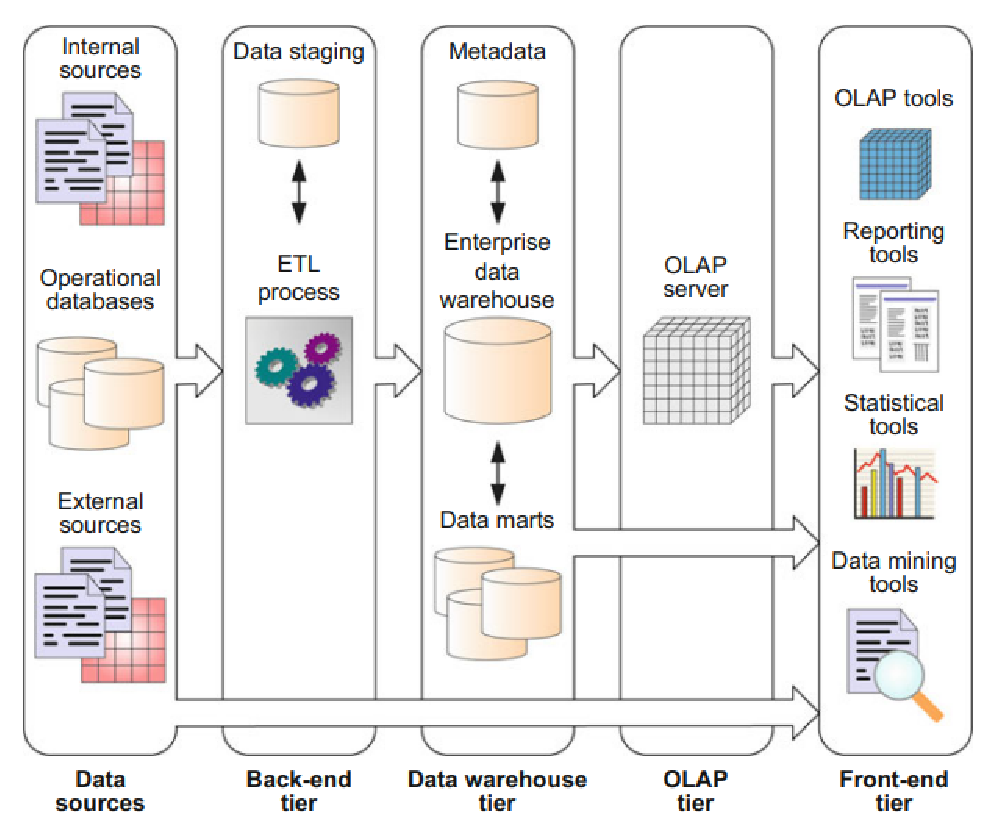
\includegraphics[width=0.8\textwidth]{figuras/typical_data_warehouse_architecture.eps}
    \caption{Arquitetura geral de um Data Warehouse}
    \label{fig:arquitetura_dw}
\end{figure}

A arquitetura apresentada é composta por quatro camadas principais:
\begin{description}
    \item[Camada de Back-End] Responsável pelos processos de extração, transformação e carga (ETL) dos dados. Aqui, os dados são extraídos 
    de fontes heterogêneas, transformados para o formato adequado e carregados no Data Warehouse. Essa camada também pode envolver o uso de 
    uma área de staging, onde os dados extraídos são temporariamente armazenados e processados antes de sua inserção no repositório central 
    de dados.
    \item[Camada do Data Warehouse] Composta pelo Data Warehouse (armazém de dados centralizado) e por Data Marts (armazéns de dados 
    especializados em áreas específicas). Além disso, essa camada inclui o repositório de metadados, que armazena informações sobre 
    a estrutura e os processos do Data Warehouse.
    \item[Camada OLAP (Online Analytical Processing)] Esta camada envolve o uso de servidores OLAP, que permitem a exploração multidimensional 
    dos dados armazenados no Data Warehouse. O OLAP facilita a análise de grandes volumes de dados de maneira interativa e flexível, utilizando 
    cubos de dados e outras estruturas analíticas.
    \item[Camada Front-End] Responsável pelas ferramentas utilizadas para análise e visualização dos dados. Inclui ferramentas OLAP, ferramentas 
    de relatórios, ferramentas estatísticas e de mineração de dados, que permitem a exploração dos dados de forma interativa e a geração de 
    insights valiosos para a tomada de decisões empresariais.
\end{description}
\cite{vaisman2014data}

\subsection{Quando Utilizar}
A implementação de um data warehouse é amplamente recomendada em contextos onde as organizações precisam tomar decisões estratégicas baseadas 
em grandes volumes de dados históricos provenientes de diversas fontes. A necessidade de analisar tendências, identificar padrões e extrair 
insights estratégicos, que não são acessíveis por meio de sistemas transacionais tradicionais, justifica a adoção dessa tecnologia.

O data warehouse desempenha um papel essencial em cenários específicos. Por exemplo, quando os dados estão dispersos em diferentes sistemas, 
o que dificulta a obtenção de uma visão unificada da organização, o data warehouse se torna uma solução eficiente. Ele possibilita a integração 
de dados de múltiplas fontes, fornecendo uma visão única e consistente das informações organizacionais. Além disso, sua capacidade de armazenar 
dados históricos permite a análise aprofundada de tendências e padrões ao longo do tempo, fator indispensável para decisões baseadas em informações 
históricas \cite{santoso2017data}.

Outro aspecto relevante é que organizações frequentemente necessitam de relatórios e análises complexas, que não podem ser gerados de forma 
eficaz por sistemas transacionais. Nesse contexto, o data warehouse, projetado especificamente para consultas e análises sofisticadas, oferece 
suporte à criação de relatórios detalhados e dashboards interativos. Ademais, ao fornecer um ambiente separado para análises, ele evita 
impactos no desempenho dos sistemas operacionais, cuja principal função é suportar as operações diárias da organização \cite{santoso2017data}.

Embora os benefícios de um data warehouse sejam inegáveis, sua implementação exige uma avaliação cuidadosa dos custos e benefícios envolvidos. 
Trata-se de um processo que pode ser complexo, demorado e custoso, requerendo investimentos significativos em infraestrutura, software e 
equipes especializadas. Apesar disso, quando bem implementado, o data warehouse pode proporcionar vantagens significativas, como a melhoria 
na qualidade da tomada de decisões, por meio do fornecimento de informações precisas e oportunas, além de ganhos em eficiência operacional, 
resultantes da otimização de processos baseada nos insights obtidos. Por fim, ele pode oferecer uma vantagem competitiva à organização, ao 
permitir análises preditivas que ajudam a antecipar tendências e oportunidades de mercado \cite{vaisman2014data, mousa2015data}.

\subsection{Quando Não Utilizar}
A implementação de um Data Warehouse, embora amplamente vantajosa em diversos contextos, apresenta limitações e desafios que podem torná-lo 
inadequado para determinados cenários. Um dos principais problemas está relacionado ao tempo e à complexidade do processo de ETL. Muitas vezes, 
os desenvolvedores não consideram adequadamente o tempo necessário para realizar essas etapas, resultando no esgotamento de grande parte do 
tempo destinado à construção do sistema. Essa situação pode gerar atrasos e custos inesperados, especialmente em projetos com cronogramas restritos.

Além disso, o modelo de design do Data Warehouse pode ser extremamente complexo e não reflexivo, dificultando sua adaptação às necessidades de 
negócios em constante mudança. Isso ocorre porque, ao adicionar novas fontes de dados ou realizar alterações nos processos, os designers do Data 
Warehouse frequentemente precisam redesenhar o ETL, resultando em modificações nas regras ou nas origens dos dados, o que aumenta a complexidade 
e o custo do sistema.

Outra limitação importante está na atualização do Data Warehouse, que geralmente é feita de forma offline. Isso significa que, enquanto o sistema 
é atualizado, as aplicações de BI não conseguem acessar os dados ou fornecer informações em tempo real. Esse atraso pode ser prejudicial para empresas 
que dependem de análises e tomadas de decisão imediatas, como em cenários de operações críticas ou de alta competitividade no mercado.

Ademais, o armazenamento de dados no Data Warehouse implica em custos adicionais. Como o Data Warehouse é uma cópia dos dados originais, ele requer um 
espaço físico maior para armazenamento, o que pode gerar custos elevados com licenciamento, manutenção e resposta a demandas de infraestrutura \cite{mousa2015data}. 

\section{Data Fabric}

A crescente proliferação de dados em formatos e plataformas diversas apresenta um desafio significativo para as organizações. A necessidade de integrar, gerenciar e
analisar esses dados de forma eficiente impulsionou a busca por soluções inovadoras. É nesse contexto que surge o conceito de Data Fabric, uma arquitetura emergente 
que visa unificar e simplificar o acesso e o uso de dados em todo o ecossistema de uma organização.
Data Fabric pode ser definida como uma estrutura unificada e flexível, independente de plataformas e tecnologias, que conecta diferentes fontes de dados, permitindo 
o acesso e a análise de forma ágil e eficiente \cite{gade2024data}. Essa arquitetura utiliza metadados para construir um conhecimento abrangente sobre os dados, 
facilitando sua descoberta, acesso e governança \cite{barik2022data}.

Em sua essência, o Data Fabric visa:
\begin{itemize}
    \item Superar os desafios dos silos de dados, integrando dados de diferentes fontes e formatos \cite{gade2024data}.
    \item Criar uma visão holística e unificada dos dados da organização \cite{barik2022data}.
    \item Simplificar o acesso e a análise de dados, permitindo que usuários de negócios acessem os dados de que precisam de forma autônoma e segura \cite{gade2024data}.
    \item Garantir a governança e a conformidade dos dados, aplicando políticas e regras de forma consistente em todo o ambiente de dados \cite{gade2024data}.
\end{itemize}

O Data Fabric representa uma mudança de paradigma na gestão de dados, evoluindo de abordagens tradicionais e fragmentadas para um modelo unificado e inteligente.

\subsection{Definição e Conceito}
O Gartner define o Data Fabric como "um conceito de design que atua como uma camada integrada (fabric) de dados e processos de conexão. Essa camada utiliza análises 
contínuas sobre metadados existentes, detectáveis e inferidos para dar suporte ao design, implantação e utilização de dados integrados e reutilizáveis em todos os 
ambientes, incluindo plataformas híbridas e multinuvem" \cite{gartner_data_fabric}. Em outras palavras, o Data Fabric visa conectar 
e fornecer uma visão holística dos ativos de dados em toda a empresa, utilizando metadados para descoberta, acesso e uso de dados de forma self-service \cite{barik2022data}.

O conceito de Data Fabric surgiu com o objetivo de conectar diferentes fontes de dados, em diferentes formatos e plataformas, de forma eficiente \cite{blohm2024data}. A ideia é criar uma 
camada de abstração que permita aos usuários acessar e analisar os dados sem se preocupar com a complexidade da infraestrutura subjacente \cite{barik2022data}.

O Data Fabric surge como uma evolução das plataformas de dados corporativos, aproveitando capacidades existentes e adicionando funcionalidades para criar uma rede 
integrada de informações. Ele não exige a consolidação física dos dados, mas utiliza metadados para conectar e permitir acesso a dados em diferentes repositórios, 
mantendo os sistemas em suas infraestruturas originais. Isso contrasta com plataformas centralizadas, que demandam a movimentação e agregação de dados em um único local \cite{barik2022data}.

\subsection{Arquitetura}
A arquitetura do Data Fabric é complexa e não existe um modelo único que atenda a todas as necessidades. No entanto, podemos identificar alguns componentes chave 
e princípios de design comuns a maioria das implementações.

Componentes da Arquitetura:
\begin{itemize}
    \item \textbf{Camada de Fontes de Dados}: O Data Fabric se conecta a uma variedade de fontes de dados, incluindo bancos de dados relacionais, bancos de dados NoSQL, data lakes, sistemas de arquivos e APIs. O Data Fabric abstrai a complexidade dessas fontes, permitindo que os usuários acessem os dados de forma uniforme, independentemente de sua localização ou formato \cite{barik2022data}.
    \item \textbf{Camada de Ingestão e Integração de Dados}: Responsável por coletar, transformar e integrar dados de diferentes fontes. O Data Fabric utiliza uma variedade de técnicas de integração de dados, como virtualização de dados, replicação de dados e ETL (Extract, Transform, Load). A escolha da técnica mais adequada depende das características dos dados, dos requisitos de desempenho e dos custos \cite{barik2022data}.
    \item \textbf{Camada de Metadados}: O Data Fabric mantém um catálogo abrangente de metadados que descrevem os dados, incluindo seu significado, relacionamento com outros dados e como podem ser usados. O Data Fabric utiliza inteligência artificial (IA) e machine learning (ML) para automatizar a descoberta, classificação e enriquecimento de metadados. Essa camada é crucial para a descoberta de dados, governança de dados e self-service \cite{barik2022data}.
    \item \textbf{Camada de Processamento e Análise de Dados}: O Data Fabric fornece um ambiente para processar e analisar dados, utilizando uma variedade de ferramentas e tecnologias, como Spark, Hadoop e plataformas de machine learning. Essa camada pode ser implementada em diferentes ambientes, como on-premises, cloud ou edge \cite{sharma2023data}.
    \item \textbf{Camada de Acesso e Consumo de Dados}: O Data Fabric fornece uma interface unificada para acessar e consumir dados, por meio de APIs, ferramentas de visualização de dados e dashboards. Essa camada permite que os usuários de negócios acessem os dados de que precisam de forma self-service, sem a necessidade de envolver a equipe de TI \cite{barik2022data}.
\end{itemize}

Princípios de Design:
\begin{itemize}
    \item \textbf{Descentralização}: O Data Fabric é uma arquitetura descentralizada, o que significa que os dados podem permanecer em seus locais originais, eliminando a necessidade de criar um repositório centralizado de dados. Isso torna o Data Fabric mais flexível e escalável \cite{sharma2023data}.
    \item \textbf{Elasticidade e Escalabilidade}: O Data Fabric é projetada para ser elástica e escalável, permitindo que as organizações adicionem ou removam recursos de computação e armazenamento conforme necessário. Isso garante que o Data Fabric possa lidar com o crescimento do volume e da variedade de dados \cite{sharma2023data}.
    \item \textbf{Segurança e Governança}: O Data Fabric implementa políticas e regras de segurança e governança de dados de forma consistente em todo o ambiente de dados, garantindo a conformidade com as regulamentações \cite{sharma2023data}.
    \item \textbf{Inteligência Artificial e Automação}: O Data Fabric utiliza IA e ML para automatizar tarefas de gerenciamento de dados, como a descoberta, classificação e enriquecimento de dados. Isso torna o Data Fabric mais eficiente e inteligente, permitindo que as organizações extraiam o máximo valor de seus dados \cite{hechler2023data}.
\end{itemize}

A arquitetura do Data Fabric é projetada para fornecer uma plataforma unificada e inteligente para gerenciar dados em todo o ecossistema de uma organização. Ao combinar 
os princípios de descentralização, elasticidade, segurança, governança e inteligência artificial, o Data Fabric capacita as organizações a aproveitar ao máximo o valor 
de seus dados, impulsionando a tomada de decisões e a inovação.

\subsection{Quando Utilizar}
Após explorar a arquitetura do Data Fabric, é crucial entender em quais cenários e situações essa abordagem se torna especialmente vantajosa. O Data Fabric não é 
uma solução universal para todos os problemas de dados, mas sim uma ferramenta poderosa que, quando aplicada corretamente, pode gerar grande valor para as organizações.

O Data Fabric é especialmente útil em organizações que enfrentam desafios na gestão de dados, como a unificação de dados altamente inter-relacionados, mas dispersos 
em diferentes sistemas. Ela atua como uma camada integradora, simplificando o acesso e análise desses dados. Além disso, ajuda a superar barreiras causadas por silos 
de dados, promovendo uma visão unificada e melhor colaboração entre equipes \cite{barik2022data}.

Empresas com múltiplas plataformas de dados, como data lakes e warehouses, podem usá-la para criar um ambiente de dados coeso e gerenciável. Sua arquitetura flexível 
e escalável permite adaptar-se rapidamente a mudanças nos requisitos de negócios, promovendo agilidade.

O Data Fabric também facilita a democratização dos dados, oferecendo suporte para análises self-service com segurança e governança adequadas. Por fim, possibilita a 
aplicação consistente de políticas de governança em todo o ambiente de dados, garantindo qualidade, segurança e conformidade de maneira automatizada. Assim, ela se 
apresenta como uma solução estratégica para integrar, gerenciar e governar dados em cenários complexos.

\subsection{Quando Não Utilizar}
Embora o Data Fabric apresente um potencial transformador para a gestão de dados em diversos cenários, existem situações em que sua implementação pode não ser a escolha 
mais adequada. A decisão de adotar uma arquitetura de Data Fabric deve ser baseada em uma análise cuidadosa das necessidades, recursos e desafios da organização.

Um dos cenários em que o Data Fabric pode não ser a melhor opção é quando organizações possui baixo volume de dados com pouca variedade, o Data Fabric podem não 
justificar o investimento e o esforço de implementação. Soluções de gerenciamento de dados mais simples e tradicionais podem ser suficientes nesses casos \cite{barik2022data}.

Outro cenário desafiador é a falta de maturidade em governança de dados. A eficácia do Data Fabric depende de processos bem estabelecidos de qualidade, segurança 
e conformidade, o que torna sua implementação mais complexa em empresas que ainda não possuem uma base sólida nesse aspecto \cite{gade2024data}.

Além disso, a adoção dessa arquitetura pode enfrentar desafios importantes. A escassez de profissionais qualificados para projetar, implementar e gerenciar sistemas 
avançados de Data Fabric pode dificultar sua implementação, levando a atrasos e à dependência de consultores externos. Além disso, a resistência cultural à mudança 
representa outro obstáculo, especialmente entre colaboradores acostumados a sistemas e processos existentes. Superar esses desafios exige uma gestão de mudanças robusta, 
que promova a compreensão dos benefícios do Data Fabric e incentive uma cultura de inovação e adaptação dentro das organizações \cite{gade2024data}.

\section{Data Lake}

Os \textbf{data lakes} são \textbf{repositórios escaláveis} projetados para armazenar \textbf{grandes volumes de dados brutos em seus formatos nativos até que sejam necessários}. Diferentemente de bancos de dados tradicionais, que lidam principalmente com dados estruturados e frequentemente escalam verticalmente, os data lakes foram concebidos para gerenciar o \textbf{volume, velocidade e variedade de dados}, incluindo dados estruturados, semiestruturados e não estruturados \cite{fang_data_lakes_2021}.

\subsubsection*{Características Principais dos Data Lakes}
\begin{itemize}
    \item \textbf{Arquitetura escalável}: Utilizam escalonamento horizontal, distribuindo a carga entre várias máquinas ou nós, o que permite gerenciar grandes volumes de dados difíceis de serem administrados em sistemas tradicionais \cite{gonzalez_scalable_systems_2019}.
    \item \textbf{Compatibilidade com tecnologias modernas}: São implementados com sistemas de arquivos distribuídos como o \textbf{HDFS} ou serviços de armazenamento em nuvem, como \textbf{Amazon S3}, \textbf{Azure Data Lake Storage Gen2} e \textbf{Google Cloud Storage} \cite{vass_bigdata_cloud_2020}.
\end{itemize}

\subsubsection*{Vantagens dos Data Lakes}
\begin{itemize}
    \item \textbf{Custo-benefício}: Aproveitam hardware comum e armazenamento em nuvem, reduzindo custos em comparação aos data warehouses tradicionais \cite{datar_lake_approaches_2020}.
    \item \textbf{Flexibilidade}: Permitem armazenar dados em formatos diversos sem a necessidade de transformações iniciais, facilitando análises futuras \cite{datar_lake_approaches_2020}.
    \item \textbf{Escalabilidade}: São projetados para crescer horizontalmente, acomodando volumes crescentes e fontes de dados variadas \cite{datar_lake_approaches_2020}.
\end{itemize}

\subsubsection*{Desvantagens dos Data Lakes}
\begin{itemize}
    \item \textbf{Confiabilidade dos dados}: Sem gestão adequada, podem se transformar em "pântanos de dados" devido à falta de controle de qualidade, gerenciamento de esquemas e proteções transacionais \cite{Architecting_data_lake_houses}.
    \item \textbf{Desempenho}: Consultas em dados brutos podem ser lentas e ineficientes \cite{Architecting_data_lake_houses}.
    \item \textbf{Complexidade de gestão}: Exigem habilidades e ferramentas especializadas para administração e segurança \cite{Architecting_data_lake_houses}.
\end{itemize}


\subsection{Tabela Comparativa: Data Lakes vs. Bancos de Dados Tradicionais}

\begin{tabular}{|p{4cm}|p{6cm}|p{6cm}|}
    \hline
    \textbf{Característica} & \textbf{Data Lakes} & \textbf{Bancos de Dados Tradicionais} \\ \hline
    Estrutura de Dados & Suporta formatos diversos (estruturados, semiestruturados e não estruturados) & Projetados para dados estruturados \\ \hline
    Escalabilidade & Escalabilidade horizontal & Escalabilidade vertical \\ \hline
    Custo & Mais econômico com uso de hardware comum e nuvem & Mais caro devido a hardware e software especializados \\ \hline
    Flexibilidade & Alta flexibilidade para diferentes formatos e esquemas & Menos flexível, requer esquemas definidos previamente \\ \hline
    Confiabilidade & Suscetível a problemas de qualidade sem gestão & Alta confiabilidade com propriedades ACID \\ \hline
\end{tabular}


\section{Data Mesh: Um Paradigma para Gestão de Dados Descentralizados}
O \textbf{Data Mesh} é uma abordagem descentralizada para a arquitetura de dados, introduzida como uma alternativa aos modelos centralizados tradicionais, como \textbf{Data Warehouses} e \textbf{Data Lakes}. Essa abordagem foca na distribuição de responsabilidades para equipes de domínio, promovendo escalabilidade e autonomia \cite{dehghani2020data}. 

\subsection{O que é Data Mesh?}
O conceito de \textit{Data Mesh} se baseia na ideia de tratar dados como produtos gerenciados por equipes de domínio, que são especialistas em seus próprios casos de uso. A arquitetura enfatiza a governança distribuída, onde os nós representam \textit{data products} e as conexões entre eles facilitam a integração \cite{akhtar2021mesh}.

\subsection{Princípios Fundamentais do Data Mesh}
O \textit{Data Mesh} baseia-se em quatro princípios fundamentais:
\begin{enumerate}
    \item \textbf{Propriedade de Dados Descentralizada e Orientada ao Domínio:} As equipes de domínio são responsáveis pelos dados que produzem, garantindo sua qualidade e acessibilidade \cite{dehghani2020data}.
    \item \textbf{Dados como Produto:} Os dados são tratados como produtos independentes, com seus próprios responsáveis que garantem governança e facilidade de consumo \cite{dehghani2020data}.
    \item \textbf{Plataforma de Dados Autossuficiente:} Uma infraestrutura centralizada abstrai a complexidade técnica, permitindo que equipes de domínio operem com eficiência \cite{akhtar2021mesh}.
    \item \textbf{Governança Federada:} Diretrizes centrais são aplicadas localmente pelas equipes, promovendo consistência e autonomia \cite{martinez2022governance}.
\end{enumerate}

\subsection{Vantagens e Desvantagens do Data Mesh}
O \textit{Data Mesh} apresenta vantagens significativas, como escalabilidade horizontal e maior agilidade organizacional. No entanto, também possui desafios, como a necessidade de equipes técnicas autônomas e de uma infraestrutura robusta para suportar a descentralização \cite{johnson2021scaling}.

\subsection{Quando Utilizar Data Mesh?}
O \textit{Data Mesh} é indicado em:
\begin{itemize}
    \item \textbf{Organizações complexas:} Grandes organizações com múltiplos domínios de dados \cite{dehghani2020data}.
    \item \textbf{Cenários de alta escalabilidade:} Empresas em rápido crescimento de volume de dados \cite{martinez2022governance}.
\end{itemize}

\subsection{Quando Não Utilizar Data Mesh?}
Evite \textit{Data Mesh} em:
\begin{itemize}
    \item \textbf{Pequenas organizações:} Onde os dados centralizados são mais fáceis de gerenciar \cite{johnson2021scaling}.
    \item \textbf{Ambientes com baixa maturidade em dados:} A descentralização pode ser excessivamente complexa \cite{akhtar2021mesh}.
\end{itemize}

\subsection{Ferramentas Open Source para Data Mesh}
Diversas ferramentas podem ser integradas ao \textit{Data Mesh}:
\begin{itemize}
    \item \textbf{Apache Airflow:} Para orquestração de pipelines de dados.
    \item \textbf{Apache Kafka:} Para ingestão e streaming de dados em tempo real.
    \item \textbf{dbt (Data Build Tool):} Para transformação e documentação de dados.
    \item \textbf{Kubernetes:} Para implantação escalável de serviços de dados \cite{smith2023tools}.
\end{itemize}

\subsection{Conclusão}
O \textit{Data Mesh} representa uma evolução na arquitetura de dados, oferecendo soluções para os desafios da centralização. No entanto, sua implementação exige uma infraestrutura bem projetada e equipes capacitadas.


\section{Apache Airflow: Orquestração de Pipelines}

O Apache Airflow é uma plataforma de orquestração de workflows de código aberto que permite programar, executar e monitorar pipelines de dados de forma programática. Desenvolvido originalmente pelo Airbnb em 2014 e posteriormente doado à Apache Software Foundation, o Airflow se tornou uma ferramenta essencial para a automação e gerenciamento de fluxos de trabalho complexos em ambientes de processamento de dados \cite{airflow_concepts}.

\subsection{Conceitos Fundamentais}

O Airflow utiliza Directed Acyclic Graphs (DAGs) para representar workflows, onde cada nó é uma tarefa e as arestas definem as dependências entre elas. Esta estrutura permite uma visualização clara do fluxo de trabalho e suas dependências, facilitando o gerenciamento e a manutenção dos pipelines \cite{garcia2021airflow}.

Os principais componentes do Airflow incluem:

\begin{itemize}
\item \textbf{DAGs (Directed Acyclic Graphs)}: Representação dos workflows como grafos direcionados acíclicos
\item \textbf{Operators}: Componentes que definem o que realmente será executado em cada tarefa
\item \textbf{Tasks}: Instâncias parametrizadas de operadores
\item \textbf{Dependencies}: Relações entre tarefas que determinam a ordem de execução
\end{itemize}

\subsection{Características Principais}

O Apache Airflow oferece diversas características que o tornam uma escolha popular para orquestração de pipelines \cite{kumar2022apache}:

\begin{enumerate}
\item \textbf{Escalabilidade}: Suporta a execução distribuída de tarefas através de workers
\item \textbf{Extensibilidade}: Permite a criação de operadores e hooks personalizados
\item \textbf{Interface Web}: Fornece uma interface intuitiva para monitoramento e gerenciamento de DAGs
\item \textbf{Versionamento}: Integra-se facilmente com sistemas de controle de versão
\item \textbf{Recuperação de Falhas}: Oferece mecanismos robustos para retry e recuperação de erros
\end{enumerate}

\subsection{Arquitetura}

A arquitetura do Airflow é composta por vários componentes que trabalham em conjunto \cite{sharma2021apache}:

\begin{itemize}
\item \textbf{Scheduler}: Responsável por agendar e disparar a execução das tarefas
\item \textbf{Executor}: Determina como as tarefas serão executadas
\item \textbf{Web Server}: Fornece a interface gráfica para interação com o sistema
\item \textbf{Metadata Database}: Armazena metadados sobre DAGs, execuções e configurações
\item \textbf{Workers}: Executam as tarefas em ambientes distribuídos
\end{itemize}

\subsection{Benefícios e Limitações}

\subsubsection{Benefícios}
\begin{itemize}
\item Configuração como código (Configuration as Code)
\item Monitoramento e logging abrangentes
\item Comunidade ativa e grande ecossistema de plugins
\item Suporte a múltiplos executores e provedores de nuvem
\end{itemize}

\subsubsection{Limitações}
\begin{itemize}
\item Complexidade inicial de configuração
\item Consumo significativo de recursos em ambientes grandes
\item Curva de aprendizado íngreme para recursos avançados
\end{itemize}

\subsection{Melhores Práticas}

Para uma utilização efetiva do Airflow, algumas práticas são recomendadas \cite{airflow_practices}:

\begin{enumerate}
\item \textbf{Atomicidade}: Criar tarefas atômicas e idempotentes
\item \textbf{Idempotência}: Garantir que múltiplas execuções produzam o mesmo resultado
\item \textbf{Documentação}: Manter documentação clara e atualizada dos DAGs
\item \textbf{Tratamento de Erros}: Implementar estratégias robustas de retry e fallback
\item \textbf{Monitoramento}: Configurar alertas e métricas adequadas
\end{enumerate}



\section{Kubernetes: Orquestração de Containers para Escalabilidade}

O Kubernetes (K8s) é uma plataforma de código aberto para orquestração de containers, originalmente desenvolvida pelo Google e posteriormente doada à Cloud Native Computing Foundation (CNCF). Esta plataforma automatiza a implantação, o dimensionamento e o gerenciamento de aplicações containerizadas, tornando-se um padrão de facto na indústria para orquestração de containers em larga escala \cite{burns2019kubernetes}.

\subsection{Arquitetura do Kubernetes}

A arquitetura do Kubernetes é baseada em um modelo master-node (também conhecido como control plane e worker nodes), onde cada componente tem responsabilidades específicas \cite{kubernetes_arch}:

\subsubsection{Control Plane (Master)}
\begin{itemize}
\item \textbf{kube-apiserver}: Expõe a API do Kubernetes e atua como frontend do cluster
\item \textbf{etcd}: Armazenamento consistente e distribuído para todos os dados do cluster
\item \textbf{kube-scheduler}: Responsável por agendar pods nos nodes do cluster
\item \textbf{kube-controller-manager}: Executa os processos de controle do cluster
\end{itemize}

\subsubsection{Worker Nodes}
\begin{itemize}
\item \textbf{kubelet}: Agente que garante que os containers estejam rodando em um pod
\item \textbf{kube-proxy}: Mantém as regras de rede nos nodes
\item \textbf{Container Runtime}: Software responsável por executar os containers
\end{itemize}

\subsection{Conceitos Fundamentais}

O Kubernetes opera com diversos conceitos fundamentais que formam a base de sua funcionalidade \cite{hightower2019kubernetes}:

\begin{enumerate}
\item \textbf{Pods}: A menor unidade implantável no Kubernetes, que pode conter um ou mais containers
\item \textbf{Services}: Abstração que define um conjunto lógico de pods e uma política de acesso
\item \textbf{Deployments}: Gerencia a criação e atualização de réplicas de pods
\item \textbf{StatefulSets}: Gerencia aplicações stateful com identidades persistentes
\item \textbf{ConfigMaps e Secrets}: Gerenciam configurações e dados sensíveis
\end{enumerate}

\subsection{Recursos de Escalabilidade}

O Kubernetes oferece diversos mecanismos para garantir a escalabilidade das aplicações \cite{luksa2021kubernetes}:

\subsubsection{Escalabilidade Horizontal}
\begin{itemize}
\item \textbf{Horizontal Pod Autoscaling (HPA)}: Ajusta automaticamente o número de pods baseado em métricas
\item \textbf{Cluster Autoscaling}: Adiciona ou remove nodes automaticamente conforme a demanda
\item \textbf{Load Balancing}: Distribui o tráfego entre múltiplas instâncias de aplicação
\end{itemize}

\subsubsection{Alta Disponibilidade}
\begin{itemize}
\item \textbf{Self-healing}: Reinicia containers que falham, substitui e reagenda containers
\item \textbf{Rolling Updates}: Permite atualizações sem downtime
\item \textbf{Multi-zone Deployment}: Distribui a carga entre diferentes zonas de disponibilidade
\end{itemize}

\subsection{Benefícios e Desafios}

\subsubsection{Benefícios}
\begin{enumerate}
\item \textbf{Portabilidade}: Funciona em qualquer ambiente (on-premise, nuvem ou híbrido)
\item \textbf{Escalabilidade}: Gerenciamento automático de recursos e carga
\item \textbf{Resiliência}: Recuperação automática de falhas
\item \textbf{Declarativo}: Configuração como código (Infrastructure as Code)
\end{enumerate}

\subsubsection{Desafios}
\begin{enumerate}
\item \textbf{Complexidade}: Curva de aprendizado íngreme
\item \textbf{Overhead Operacional}: Requer equipe especializada para manutenção
\item \textbf{Custos}: Pode ser dispendioso em ambientes pequenos
\item \textbf{Segurança}: Requer atenção especial à configuração de segurança
\end{enumerate}

\subsection{Melhores Práticas}

Para uma implementação efetiva do Kubernetes, algumas práticas são recomendadas \cite{arundel2021kubernetes}:

\begin{itemize}
\item \textbf{Segurança}: Implementar políticas de segurança e network policies
\item \textbf{Monitoramento}: Utilizar ferramentas como Prometheus e Grafana
\item \textbf{Logging}: Centralizar logs com soluções como ELK Stack
\item \textbf{Resource Management}: Definir limites e requisitos de recursos
\item \textbf{Backup}: Implementar estratégias de backup e disaster recovery
\end{itemize}




\section{FastAPI: Desenvolvimento de APIs para Integração de Dados}

FastAPI é um framework moderno e de alto desempenho para construção de APIs com Python, baseado em padrões como OpenAPI (anteriormente conhecido como Swagger) e JSON Schema. Desenvolvido por Sebastián Ramírez, o FastAPI se destaca por sua velocidade de execução, facilidade de uso e geração automática de documentação interativa \cite{fastapi_foundation}.

\subsection{Características Fundamentais}

O FastAPI possui características que o tornam particularmente adequado para integração de dados \cite{ramirez2022fastapi}:

\begin{enumerate}
\item \textbf{Performance}: Baseado no ASGI (Asynchronous Server Gateway Interface) e no Starlette
\item \textbf{Tipagem Estática}: Utiliza type hints do Python para validação automática
\item \textbf{Documentação Automática}: Gera documentação interativa OpenAPI e ReDoc
\item \textbf{Async/Await}: Suporte nativo a programação assíncrona
\item \textbf{Validação de Dados}: Baseada no Pydantic para validação e serialização
\end{enumerate}

\subsection{Arquitetura e Componentes}

A arquitetura do FastAPI é construída sobre componentes modernos e eficientes \cite{kumar2023modern}:

\subsubsection{Componentes Principais}
\begin{itemize}
\item \textbf{Starlette}: Framework ASGI leve para aplicações assíncronas
\item \textbf{Pydantic}: Biblioteca para validação de dados usando type annotations
\item \textbf{Uvicorn}: Servidor ASGI de alto desempenho
\item \textbf{OpenAPI}: Especificação para documentação de APIs RESTful
\end{itemize}

\subsection{Integração de Dados com FastAPI}

O FastAPI oferece recursos robustos para integração de dados \cite{wilson2023data}:

\subsubsection{Modelos de Dados}
\begin{verbatim}
from pydantic import BaseModel

class DataModel(BaseModel):
id: int
name: str
value: float
\end{verbatim}

\subsubsection{Endpoints para Manipulação de Dados}
\begin{itemize}
\item \textbf{CRUD Operations}: Implementação simplificada de operações básicas
\item \textbf{Batch Processing}: Processamento eficiente de grandes conjuntos de dados
\item \textbf{Streaming}: Suporte a streaming de dados em tempo real
\item \textbf{Background Tasks}: Processamento assíncrono de tarefas pesadas
\end{itemize}

\subsection{Segurança e Autenticação}

FastAPI oferece diversos mecanismos de segurança \cite{brown2023securing}:

\begin{enumerate}
\item \textbf{OAuth2}: Suporte nativo a OAuth2 com diferentes fluxos
\item \textbf{JWT}: Integração com JSON Web Tokens
\item \textbf{API Keys}: Autenticação via chaves de API
\item \textbf{CORS}: Configuração flexível de Cross-Origin Resource Sharing
\end{enumerate}

\subsection{Performance e Escalabilidade}

O FastAPI se destaca em termos de performance \cite{performance_metrics}:

\subsubsection{Métricas de Desempenho}
\begin{itemize}
\item Baixa latência em requisições HTTP
\item Alta capacidade de processamento concorrente
\item Uso eficiente de recursos computacionais
\item Excelente desempenho em operações I/O-bound
\end{itemize}

\subsection{Melhores Práticas}

Para um desenvolvimento eficiente com FastAPI, recomenda-se \cite{martinez2023best}:

\begin{enumerate}
\item \textbf{Estruturação do Projeto}
\begin{itemize}
\item Organização modular do código
\item Separação clara de responsabilidades
\item Uso de dependency injection
\end{itemize}

\item \textbf{Tratamento de Erros}
\begin{itemize}
    \item Implementação de exception handlers
    \item Respostas de erro padronizadas
    \item Logging adequado
\end{itemize}

\item \textbf{Documentação}
\begin{itemize}
    \item Documentação clara dos endpoints
    \item Exemplos de uso
    \item Descrições detalhadas dos modelos de dados
\end{itemize}

\end{enumerate}

\subsection{Limitações e Considerações}

Apesar de suas vantagens, é importante considerar algumas limitações \cite{kumar2023modern}:

\begin{itemize}
\item Necessidade de conhecimento em programação assíncrona
\item Curva de aprendizado para recursos avançados
\item Complexidade adicional em projetos muito grandes
\item Dependência do ecossistema Python
\end{itemize}


\section{Pipelines de Dados no Diagnóstico de Câncer de Pele}

O desenvolvimento de pipelines de dados para o diagnóstico de câncer de pele representa uma interseção crucial entre a engenharia de dados e a medicina. Estes pipelines são projetados para processar, analisar e gerenciar grandes volumes de imagens dermatológicas, auxiliando no diagnóstico precoce e preciso de diferentes tipos de câncer de pele \cite{zhang2021deep}.

\subsection{Arquitetura do Pipeline}

A arquitetura de um pipeline de dados para diagnóstico de câncer de pele tipicamente inclui várias etapas interconectadas \cite{esteva2022deep}:

\begin{enumerate}
\item \textbf{Aquisição de Dados}
\begin{itemize}
\item Captação de imagens dermatológicas
\item Digitalização de prontuários médicos
\item Metadados clínicos associados
\end{itemize}
\item \textbf{Pré-processamento}
\begin{itemize}
    \item Normalização de imagens
    \item Remoção de ruídos
    \item Segmentação de lesões
    \item Augmentação de dados
\end{itemize}

\item \textbf{Processamento}
\begin{itemize}
    \item Extração de características
    \item Análise de textura e cor
    \item Classificação de lesões
\end{itemize}

\item \textbf{Armazenamento e Recuperação}
\begin{itemize}
    \item Banco de dados de imagens
    \item Sistema de cache
    \item Backup e redundância
\end{itemize}
\end{enumerate}

\subsection{Componentes Essenciais}

Os componentes fundamentais do pipeline incluem \cite{kumar2023medical}:

\subsubsection{Infraestrutura de Dados}
\begin{itemize}
\item \textbf{Storage Layer}: Armazenamento distribuído para grandes volumes de imagens
\item \textbf{Processing Layer}: Recursos computacionais para processamento de imagens
\item \textbf{Analytics Layer}: Ferramentas para análise e visualização
\end{itemize}

\subsubsection{Modelos de Processamento}
\begin{itemize}
\item \textbf{Redes Neurais Convolucionais (CNN)}
\item \textbf{Algoritmos de Segmentação}
\item \textbf{Modelos de Classificação}
\end{itemize}

\subsection{Fluxo de Dados e Processamento}

O fluxo de dados em um pipeline de diagnóstico de câncer de pele segue um processo estruturado \cite{wang2023automated}:

\begin{enumerate}
\item \textbf{Ingestão de Dados}
\begin{itemize}
\item Coleta de imagens dermatoscópicas
\item Validação de qualidade da imagem
\item Padronização de formato
\end{itemize}
\item \textbf{Pré-processamento de Imagens}
\begin{itemize}
    \item Normalização de contraste e brilho
    \item Remoção de artefatos
    \item Segmentação da região de interesse
\end{itemize}

\item \textbf{Análise e Classificação}
\begin{itemize}
    \item Extração de características
    \item Aplicação de modelos de ML/DL
    \item Geração de predições
\end{itemize}
\end{enumerate}

\subsection{Garantia de Qualidade}

A qualidade dos dados é crucial para o diagnóstico preciso \cite{smith2023quality}:

\begin{itemize}
\item \textbf{Controle de Qualidade de Imagem}
\begin{itemize}
\item Verificação de resolução
\item Análise de contraste
\item Validação de formato
\end{itemize}

\item \textbf{Validação de Dados}
\begin{itemize}
    \item Verificação de completude
    \item Consistência de metadados
    \item Integridade dos dados
\end{itemize}
\end{itemize}

\subsection{Desafios e Considerações}

O desenvolvimento de pipelines para diagnóstico de câncer de pele enfrenta diversos desafios \cite{chen2023challenges}:

\begin{enumerate}
\item \textbf{Desafios Técnicos}
\begin{itemize}
\item Variabilidade na qualidade das imagens
\item Necessidade de processamento em tempo real
\item Requisitos de armazenamento
\end{itemize}
\item \textbf{Desafios Clínicos}
\begin{itemize}
    \item Variabilidade das lesões
    \item Necessidade de alta precisão
    \item Interpretabilidade dos resultados
\end{itemize}

\item \textbf{Considerações Éticas}
\begin{itemize}
    \item Privacidade dos pacientes
    \item Segurança dos dados
    \item Conformidade regulatória
\end{itemize}
\end{enumerate}

\section{Fluxo de Dados em Arquitetura de Data Fabric}

Em uma arquitetura de Data Fabric, o fluxo de dados é projetado para proporcionar uma integração contínua e inteligente de dados através de múltiplos ambientes, garantindo consistência, governança e acessibilidade \cite{sharma2023data}. Este modelo representa uma evolução significativa na forma como as organizações gerenciam e utilizam seus dados, especialmente em ambientes híbridos e distribuídos.






\subsection{Componentes do Fluxo de Dados}

O fluxo de dados em uma arquitetura Data Fabric é composto por diversos componentes interconectados \cite{hechler2023data}:

\begin{enumerate}
\item \textbf{Camada de Ingestão}
\begin{itemize}
\item Conectores de fonte de dados
\item Mecanismos de streaming
\item APIs de integração
\item Protocolos de comunicação
\end{itemize}

\item \textbf{Camada de Processamento}
\begin{itemize}
    \item Transformação de dados
    \item Validação e limpeza
    \item Enriquecimento de dados
    \item Normalização
\end{itemize}

\item \textbf{Camada de Armazenamento}
\begin{itemize}
    \item Data Lakes
    \item Data Warehouses
    \item Bancos de dados distribuídos
    \item Sistemas de cache
\end{itemize}
\end{enumerate}

\subsection{Padrões de Fluxo de Dados}

Os padrões de fluxo de dados em uma arquitetura Data Fabric podem ser categorizados em diferentes tipos \cite{blohm2024data}:

\subsubsection{Fluxo Batch}
\begin{itemize}
\item Processamento em lotes programados
\item Transformações complexas
\item Agregações de grande escala
\item Cargas incrementais
\end{itemize}

\subsubsection{Fluxo Real-time}
\begin{itemize}
\item Streaming de dados
\item Processamento em tempo real
\item Análise contínua
\item Alertas e notificações
\end{itemize}

\subsubsection{Fluxo Híbrido}
\begin{itemize}
\item Combinação de batch e real-time
\item Processamento lambda
\item Análise preditiva
\item Detecção de anomalias
\end{itemize}

\subsection{Gestão e Controle do Fluxo}

A gestão eficiente do fluxo de dados é crucial para o sucesso da arquitetura \cite{gade2024data}:

\begin{enumerate}
\item \textbf{Orquestração}
\begin{itemize}
\item Agendamento de jobs
\item Gerenciamento de dependências
\item Controle de concorrência
\item Recuperação de falhas
\end{itemize}
\item \textbf{Monitoramento}
\begin{itemize}
    \item Métricas de performance
    \item Logs de execução
    \item Rastreamento de dados
    \item Alertas de anomalias
\end{itemize}

\item \textbf{Governança}
\begin{itemize}
    \item Políticas de acesso
    \item Compliance
    \item Qualidade dos dados
    \item Lineage de dados
\end{itemize}
\end{enumerate}

\subsection{Integração e Interoperabilidade}

A integração eficiente é fundamental para o sucesso do Data Fabric \cite{barik2022data}:

\begin{itemize}
\item \textbf{Conectividade}
\begin{itemize}
\item APIs padronizadas
\item Protocolos de comunicação
\item Adaptadores de fonte de dados
\end{itemize}
\item \textbf{Transformação}
\begin{itemize}
    \item Mapeamento de dados
    \item Conversão de formatos
    \item Normalização de esquemas
\end{itemize}

\item \textbf{Sincronização}
\begin{itemize}
    \item Consistência de dados
    \item Replicação
    \item Resolução de conflitos
\end{itemize}
\end{itemize}

\subsection{Desafios e Considerações}

A implementação do fluxo de dados em Data Fabric apresenta diversos desafios \cite{addagada2022best}:

\begin{enumerate}
\item \textbf{Técnicos}
\begin{itemize}
\item Complexidade da infraestrutura
\item Latência em ambientes distribuídos
\item Escalabilidade
\end{itemize}
\item \textbf{Operacionais}
\begin{itemize}
    \item Manutenção contínua
    \item Gerenciamento de recursos
    \item Resolução de problemas
\end{itemize}

\item \textbf{Organizacionais}
\begin{itemize}
    \item Adaptação cultural
    \item Capacitação de equipes
    \item Gestão de mudanças
\end{itemize}
\end{enumerate}


\section{Ingestão de Dados e Preprocessamento de Imagens}

A ingestão de dados e o preprocessamento de imagens são etapas cruciais em sistemas de análise de imagens médicas, especialmente no contexto do diagnóstico de câncer de pele. Estas etapas estabelecem a base para análises posteriores e influenciam diretamente a qualidade dos resultados obtidos \cite{garcia2023medical}.

\subsection{Ingestão de Dados}

O processo de ingestão de dados envolve a coleta e integração de diferentes tipos de dados médicos \cite{kumar2023data}:

\subsubsection{Fontes de Dados}
\begin{itemize}
\item \textbf{Imagens Dermatoscópicas}
\begin{itemize}
\item Fotografias clínicas de alta resolução
\item Imagens microscópicas digitalizadas
\item Imagens termográficas
\end{itemize}

\item \textbf{Dados Clínicos Associados}
\begin{itemize}
    \item Histórico médico do paciente
    \item Diagnósticos anteriores
    \item Metadados das imagens
\end{itemize}
\end{itemize}

\subsection{Preprocessamento de Imagens}

O preprocessamento é fundamental para garantir a qualidade e padronização das imagens \cite{smith2023image}:

\begin{enumerate}
\item \textbf{Normalização de Imagens}
\begin{itemize}
\item Ajuste de contraste
\item Correção de brilho
\item Padronização de tamanho
\item Normalização de cores
\end{itemize}

\item \textbf{Técnicas de Aprimoramento}
\begin{itemize}
    \item Redução de ruído
    \item Realce de bordas
    \item Correção de iluminação
    \item Filtros de suavização
\end{itemize}

\item \textbf{Segmentação}
\begin{itemize}
    \item Identificação da região de interesse
    \item Separação lesão/pele saudável
    \item Remoção de artefatos
\end{itemize}
\end{enumerate}

\subsection{Pipeline de Processamento}

O pipeline de processamento segue uma sequência estruturada de operações \cite{wang2023automated}:

\begin{figure}[h]
\centering
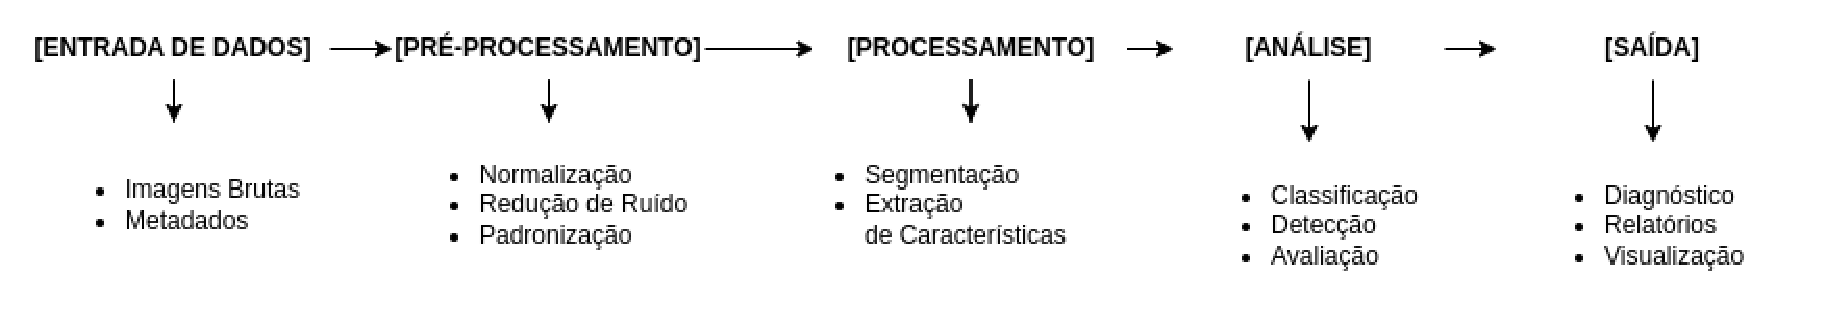
\includegraphics[width=0.8\textwidth]{figuras/pipeline_processamento.eps}
\caption{Pipeline de Processamento de Imagens Dermatológicas}
\label{fig:pipeline_proc}
\end{figure}

\subsubsection{Etapas do Pipeline}
\begin{enumerate}
\item \textbf{Validação Inicial}
\begin{itemize}
\item Verificação de formato
\item Controle de qualidade
\item Validação de metadados
\end{itemize}

\item \textbf{Preprocessamento Básico}
\begin{itemize}
    \item Redimensionamento
    \item Normalização
    \item Conversão de formato
\end{itemize}

\item \textbf{Preprocessamento Avançado}
\begin{itemize}
    \item Segmentação
    \item Extração de características
    \item Augmentação de dados
\end{itemize}
\end{enumerate}

\subsection{Técnicas de Augmentação de Dados}

A augmentação de dados é essencial para melhorar o treinamento de modelos \cite{zhang2023augmentation}:

\begin{itemize}
\item \textbf{Transformações Geométricas}
\begin{itemize}
\item Rotação
\item Reflexão
\item Escala
\item Translação
\end{itemize}

\item \textbf{Transformações de Intensidade}
\begin{itemize}
    \item Ajuste de contraste
    \item Mudança de brilho
    \item Ruído gaussiano
    \item Alteração de saturação
\end{itemize}
\end{itemize}

\subsection{Controle de Qualidade}

O controle de qualidade é fundamental durante todo o processo \cite{chen2023quality}:

\begin{enumerate}
\item \textbf{Métricas de Qualidade}
\begin{itemize}
\item Resolução da imagem
\item Relação sinal-ruído
\item Nitidez
\item Contraste
\end{itemize}

\item \textbf{Validação}
\begin{itemize}
    \item Verificação automática
    \item Revisão manual
    \item Testes de consistência
\end{itemize}
\end{enumerate}